\chapter{Experiment}
\label{cha:experi}

For the experiment, we use spark framework to implement our model. In this chapter, we will firstly introduce some knowledge about spark and how we use these techniques to implement our model. After that, we will introduce the experiments we did and analysis our results.


\section{Spark}

Spark has one driver and several executors. Usually, an executor is a cpu core, and we call each machine as worker, so each worker has several executors. But logically we only need the driver and the executors, only for something about tuning we should care about the worker stuff, e.g. some operations need to do communication between different machine. But for most of cases, each executor just fetch part of data and deal with it, and then the driver collect data from all executors.\\

Spark has many useful things. What I use are about RDD (Resilient Distributed Datasets) and some operations on RDD, which is a special data structure containing the data set. and is convenient to be These operations have two type, one is Transformation operation, another is action operation. Firstly, Spark reads text file from file system (normally it is HDFS). And now, the data is the form of RDD. The transformation operation is to transform a RDD to another RDD. RDD has two types, the one read from file system is called HDFS RDD, the one transformed by transformation operation is called map RDD. Generally after some transformation operations, people use the action operation to gain some useful information from the last RDD. To be noted that, transformation is not to change the element in the current RDD, insead it create a new RDD. How about the old one? If you really need it, you can store it in catch, memory or the disk. Some times we store it (catch it) not only for the intermediate results, but also for some algorithms required iteration. For instance, if you want to use action operation to gain some 
Transformation operation is mainly about map and filter, which is very similar as the operations in any functional programming. And the action operation is mainly about aggregate, reduce, count, and collect. RDD can be operated only by transformation operation and stored logically in every executor. Data in RDD can not be changed. Spark use some operations to Each transformation operation will create a new RDD and would not change the DATA in the original RDD.

\section{Implementation}

We use $syn0$ to represent the input embedding $V$ and $syn1$ to represent the output embedding $U$. $syn0$ and $syn1$ are set to be as the broadcast variables, which is only readable and can not be changed by executors.

\paragraph{Assign Step}\ \\
In the assignment, we use map transformation to transform each sentence with senses information to another sentence with changed senses information. So one RDD becomes to another RDD. In this process, $syn0$ and $syn1$ will be used (only read) to calculate the loss. 

\paragraph{Learn Step}\ \\
In the training, we also use map transformation. Instead of transforming sentences to sentences, we transform the original sentence RDD into the collection of updated $syn0$ and updated $syn1$. Yes, we update $syn0$ and $syn1$ in this process, because we need to train our parameters. But executors can really change the $syn0$ and $syn1$ directly. So we copy these broadcast variables to the local $syn0$ and $syn1$ in each executor, so that each executor has its own $syn0$ and $syn1$ and update them independently. And then we use the average of them as the new global $syn0$ and $syn1$.\\

So each executor has two vectors (representing $syn0$ and $syn1$ respectively). And then we use $treeAggregate$ to collect all such vectors together from different executor (cpu core).  In the aggregation, different $syn0$'s vectors add up together, and different $syn0$'s vectors add up together. Finally, we get one $syn0$ and one $syn1$. For now, we set them as new $syn0$ and $syn1$, which will be used as the broadcast value in the next iteration. \\

After getting the new global $syn0$ and $syn1$, because they are added up by several ones, some values of some embeddings may be very big. Thus, we need to do normalization to avoid to big values. Our normalization method is very simple, which is to check all embeddings from $syn0$ and $syn1$ if the length is bigger than 4, if that we just normalization them to the new embeddings with length of 4.\\


\section{Experiment}

\paragraph{Data preparing} \ \\
We use the same corpus as other papers used, a snapshot of Wikipedia at April, 2010 (Shaoul, 2010), which has 990 million tokens. Firstly we count the all words in the corpus. We transform all words to lower capital and then generate our vocabulary (dictionary). Actually, we set a $minCount$, if the word count is smaller than this value. We remove it from corpus, so it won't be in the vocabulary. And then we calculate the frequency of word count. For example, there are 300 words which has count 10. So the frequency of count 10 is 300. After that, we can calculate the accumulated frequency, which can help us to choose the $minCount$. That is, if accumulated frequency of count 200 is 100000, there would be 100000 words whose count is at least 200. So we can adjust the different accumulated frequency to get different vocabulary size.

\paragraph{Environment} \ \\
Our program is running on a single machine with 32 cores. For some experiment, we use all cores as executers. We also tried some experiments on several machine, but that is not very good for our program, we will explain some reasons later. So there is no communication between different machines.  But there are some experiments requiring fewer cores.

\paragraph{Training set and validation set} \ \\
We split corpus as training set and validation set. Training set has $99\%$ data and validation set has only $1\%$ data. We use validation set to monitor our training process if it is convergence. If an training algorithm is convergence, the loss of validation set should be at the lowest value. And then it will gradually increase, which means the training is over-fitting. So we will calculate the loss of validation set every several training iterations and then compare with the previous validation loss, if the current value is bigger than previous value, we stop our training process and fetch the previous result as the final result to store into the disk. That is, after each calculating the loss of validation set, we will store our results, and we won't do anything in the step to stop. \\

To be noted that, because we want to use the validation set to monitor our training, so the validation set and training set should not be overlapping. And another import thing is that, the negative samplings of validation set should always be fixed.  The assignment step for validation set is almost same as the one for training set. The only different thing is that, the negative samples for each word of each sentence in the validation set is not changed. But for each iteration of assignment for sentence in training set, the negative sampling are new. \\

Actually, for our cases, it is not very easy to choose the vocabulary size and the vector size. For each experiment, we record the $count$ time and $treeAggregate$ time. It is also difficult to choose the number of RDD, which although is not the very important factor to decide the final results. We found that the number of RDDs only affect the time and space using, it would not affect the final loss.

We need two steps to train sense embedding vectors. The first step is to set the number of sense only one and train normal word embedding vectors. In second step, the program will use the result from the first step to do initialization and then train the sense embedding vectors.

We did four different experiments for the first step shown as \ref{tab:experiment4}, based on that we did another 9 experiments for the second step \ref{tab:experiment9}. For these two tables, we give another notation table as \ref{tab:notation} to explain the meaning of each label. Considering other parameters like the number of RDDs and window size is always fixed. The The difference for parameters between step 1 and step 2 is that, 


\begin{table}[H]
\begin{center}
\begin{tabular}{|l|l|}
\hline
id & The id number of the experiment. \\ \hline
c1 &  Min count for involving in Vocabulary\\ \hline
vec & Vector size for each embedding vector\\ \hline
cm &  Threshold array for different number of senses\\ \hline
lr &  The learning rate at the beginning of the experiment.\\ \hline
gm &  The reduction rate of learning rate for each iteration\\ \hline
syn1 & Whether each word has only one output embedding vector\\ \hline
\multirow{2}{*}{t1} 
& The average Training time of each iteration \\ 
&(excluding the parameter collection.\\ \hline
t2 & The average treeAggregate operation time of each iteration \\ \hline
iter & The number of training iterations \\ \hline
\multirow{2}{*}{t3} 
&The average time of each iteration \\
&(including Assign step, train step and parameters collection) \\ \hline

t4 & Total training time \\ \hline
loss & The best loss of validation set \\ \hline
SCWS & The Spearman’s rank correlations on SCWS dataset. \\ \hline
word353 & The Spearman’s rank correlations on word353 dataset \\ \hline
\multirow{2}{*}{init} 
& The id number of experiment in step 1 \\
&(used to initialize embedding vectors)\\
\hline
\end{tabular}
\caption{Notation explaination for parameters evaluation } \label{tab:notation}
\end{center}
\end{table}

\begin{table}[H]
\begin{center}
\begin{tabular}{|l|l|}
\hline
numRDD=20 & The number of RDD to split training data set.\\ \hline
 windowSize=5& The window size  \\ \hline
 numNegative=10& \\ \hline
 &  \\ \hline

\hline
\end{tabular}
\caption{Fixed value} \label{tab:fixvalue}
\end{center}
\end{table}


\begin{table}[H]

\begin{center}
\begin{tabular}{|l|l|l|l|l|}
\hline
id&c1&vec&lr&gm \\ \hline
(1) 	&  200 		& 300  	& 0.1		& 0.9	\\ \hline
(2) 	&  200 		& 250  	& 0.1		& 0.9	\\ \hline
(3) 	&  200 		& 200  	& 0.1		& 0.9	\\ \hline
(4) 	&  200 		& 150  	& 0.1		& 0.9	\\ \hline
(5) 	&  200 		& 100  	& 0.1		& 0.9	\\ \hline
(6) 	&  200 		& 50 	& 0.1		& 0.9	\\ \hline
(7)	&  20		& 50	& 0.1		& 0.9	\\ \hline
(8)	&  20		& 50	& 0.01		& 0.95	\\ \hline
\end{tabular}

\caption{5 Different Experiments in Step 1} \label{tab:experiment4}
\end{center}
\end{table}


\begin{table}[H]

\begin{center}
\begin{tabular}{|l|l|l|l|l|l|l|l|}
\hline
id&c1&vec&cm&lr&gm&syn1&init \\ \hline
1 	&  200 		& 300 	& 2000$\_$10000 	& 0.1		& 0.9	& true & (1)\\ \hline
2	&  200		& 250   & 2000$\_$10000 	& 0.1		& 0.9	& true & (2)\\ \hline
3	&  200		& 200   & 2000$\_$10000 	& 0.1		& 0.9	& true & (3)\\ \hline
4	&  200		& 150   & 2000$\_$10000 	& 0.1		& 0.9	& true & (4)\\ \hline
5 	&  200 		& 100 	& 2000$\_$10000 	& 0.1		& 0.9	& true & (5) \\ \hline
6 	&  200 		& 50 	& 2000$\_$10000 	& 0.1		& 0.9	& true & (6)\\ \hline
7	&  20		& 50	& 2000$\_$10000	& 0.1		& 0.9	& true & (7)\\ \hline
8	&  20		& 50	& 2000$\_$10000	& 0.01		& 0.95	& true & (8)\\ \hline
9 	&  20		& 50 	& 2000$\_$100000 	& 0.1		& 0.9	& true & (7)\\ \hline
10 	&  20		& 50 	& 7000$\_$10000 	& 0.1		& 0.9	& true & (7)\\ \hline
11 	&  20		& 50 	& 2000$\_$10000 	& 0.1		& 0.9	& false& (7)\\ \hline
\end{tabular}

\caption{9 Different Experiments in Step 2} \label{tab:experiment9}
\end{center}
\end{table}

\section{Evaluation}

In the following analysis, we use three different methods to assistant to our works. Nearest Neighbours, Similarity Task including WordSim-353 [] Dataset and the Contextual Word Similarity (SCWS) dataset from Huang[], and t-SNE based Visualization. 

WordSim-353 Dataset is a Dataset made up by 353 pairs of words following by similarity scores from 10 different people and an average score. SCWS Dataset has 2003 pairs with their context respectively, which also contains 10 scores from 10 different people and an average score. 

For the WordSim-353 dataset, we use the maxSim function to calculate the similarity score of two words from our model as following:
$$maxSim(w,w^\prime)=max\{Cosine(V_{w,i},V_{w^\prime,j})\}, (1\leq i\leq N_w, 1\leq j\leq N_{w^\prime} ) $$
where $Cosine(x, y)$ denotes the cosine similarity score of vector x and y. And as the same notation from last chapter, $N_w$ means the number of senses for word $w$, and $V_{w,i}$ represents the $i$-th sense input embedding vectors of word $w$. 

For the SCWS dataset, it is similar as the \textbf{Assign} operation, we use center word to predict the context words. But here we do not do the real assignment for whole sentence which needs several times to assign until it is stable. Actually, our sense output embedding has only one sense. So we just use the normal skip-gram model's prediction function to select the best center word's sense.
\subsection{Parameters Comparison}

Different parameters and hyper parameter can generate different loss and spend different time and memory space. Totally we did 9 experiments as following. In the early version , we try many different parameters on the small dataset and found that the number of negative samples, the window size are not the typical factors to affect the final results. And we also found that it is better to choose $numRDDs$ = 20, which can balance the $count$ time and $treeAggregate$ time. Unfortunately, we lost some data of these early experiments. So in this section we only compare the following different experiments. \\

In the following, we will fix some parameters and build 5 comparison groups based these 9 experiments to check how different parameters affect the final validation loss, the convergence speed, training time and similarity results. Table \ref{tab:experiment9} show the different 

\paragraph{Different vector size} \ \\
From the comparison in Table \ref{tab:group1} , it is clear that the vector size is not the key factor to affect the final loss, even though the loss from experiment 3 is a little better. And there is another interesting thing that, when vector size if bigger, the score from SCWS is better but the score from word353 is worse. 
\begin{table}[H]

\begin{center}
\begin{tabular}{|l|l|l|l|l|l|l|l|l|l|}
\hline
id& vec  & t1 & t2 & iter & t3 & t4 &   loss  & 	SCWS & 	word353	   \\ 
\hline
1 	& 300 	& 947.8	& 842	& 35	& 2272.9 &	79550  & 0.2437 &0.5048 & 0.5233  \\ 
\hline
2 	& 250 	& 764.7& 533	& 35	& 1755.7 &	61450  & 0.2437 &0.5083 & 0.5271 \\ 
\hline
3 	& 200 	& 632.5& 322	& 40	& 1389.9 &  55593  & 0.2436 &0.5103 & 0.5371 \\ 
\hline
4 	& 150 	& 502.7& 210	& 35	& 1069.9 &	37448  & 0.2440 &0.5048 & 0.5233 \\ 
\hline
5 	& 100 	& 494.7	& 70.1	& 35	& 827.30 &	28956  & 0.2446 &0.4994 & 0.5355  \\ 
\hline
6 	& 50 	& 342.9& 34.6	& 35	& 683.29 &	23915  & 0.2458 &0.4666 & 0.5449  \\ 
\hline
\end{tabular}
\caption{Different Vector Size Comparison} \label{tab:group1} 
\end{center}
\end{table}


\begin{figure}[!ht]
  \centering
	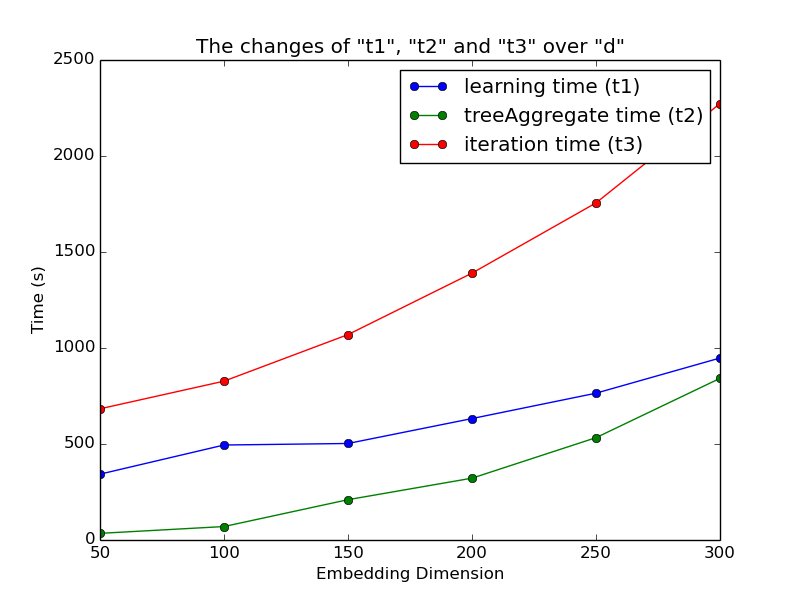
\includegraphics[width=0.8\textwidth]{vectime} 
	\caption{Shows the effect of varying embedding dimensionality of our Model on the Time}
	\label{fig:vec_time}
\end{figure}

\begin{figure}[!ht]
  \centering
	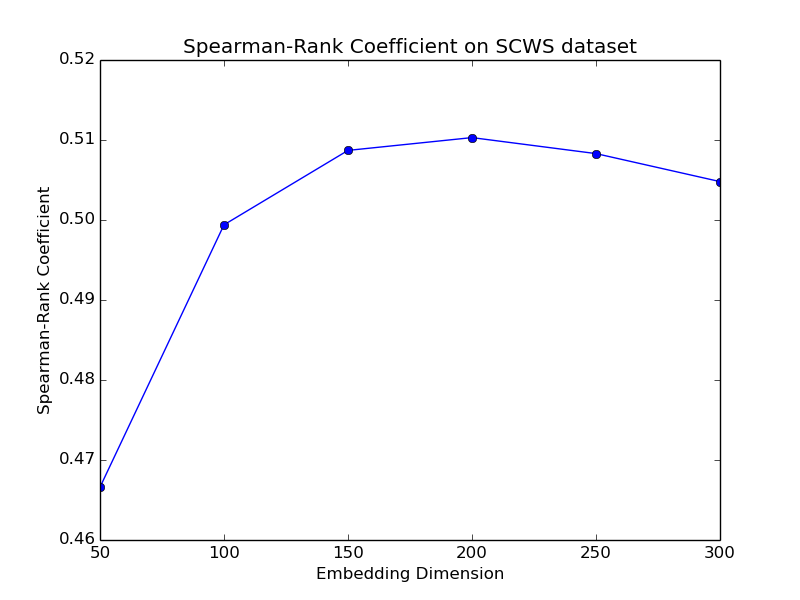
\includegraphics[width=0.7\textwidth]{vecSCWS} 
	\caption{Shows the effect of varying embedding dimensionality of our Model on the SCWS task}
	\label{fig:vec_SCWS}
\end{figure}


\begin{figure}[!ht]
  \centering
	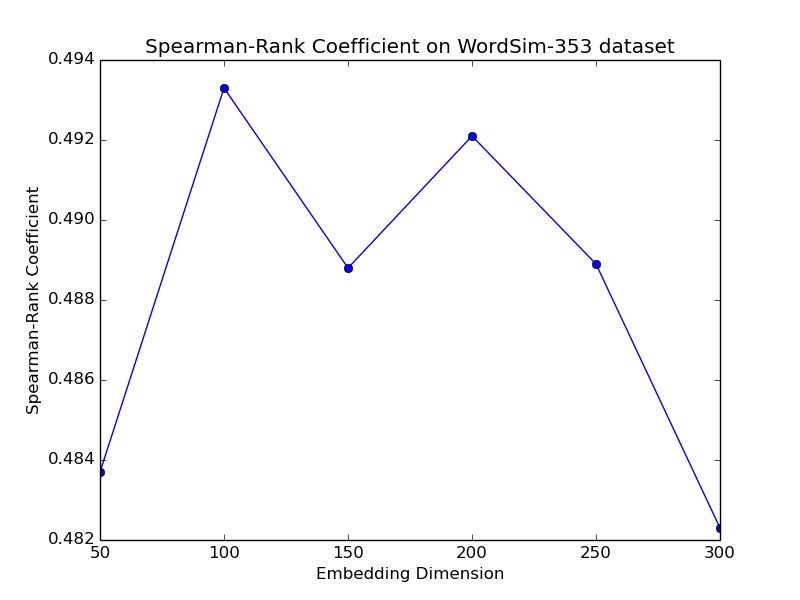
\includegraphics[width=0.7\textwidth]{vecword353} 
	\caption{Shows the effect of varying embedding dimensionality of our Model on the word353 task}
	\label{fig:vec_word353}
\end{figure}




\paragraph{Different Min Count} \ \\
We can find from Table \ref{tab:group2} , the size of dictionary is not the important factor based on loss or similarity tasks. Min count is used to remove some words which is not frequent. As we know , each word's embedding vector is trained based on the surrounding words. Since those words are infrequent, each of them involve the training of frequent words very few. So they won't affect the final embedding vectors of frequent words.

\begin{table}[H]
\caption{Different Min Count Comparison} \label{tab:group2} 
\begin{center}
\begin{tabular}{|l|l|l|l|l|l|l|l|l|l|}
\hline
id& c1 & t1 & t2 & iter & t3 & t4 & loss & SCWS & word353	   \\ 
\hline
6 	&  200 	& 342.9	& 34.6	& 35	& 683.3 &	23915  & 0.2458 &0.4666 & 0.5449  \\ 
\hline
7	&  20	& 849.0	& 343	& 35	& 1838.1 &	64335  & 0.2457 &0.4371	&0.4891    \\ 
\hline
\end{tabular}
\end{center}
\end{table}

\paragraph{Different Sense Count Comparison} \ \\
From Table \ref{tab:group3} tell us ...

\begin{table}[H]
\caption{Different Sense Count Comparison} \label{tab:group3} 
\begin{center}
\begin{tabular}{|l|l|l|l|l|l|l|l|l|l|}
\hline
id& cm & t1 & t2 & iter & t3 & t4 &    loss  & 	SCWS & 	word353	   \\ 

\hline
7	& 2000$\_$10000	& 849	& 343	& 35	& 1838 &	64335  & 0.2457 &0.4371	&0.4891	  \\ 
\hline
9 	& 2000$\_$100000 	& 798	& 338	& 35	& 1712 &	59912  & 0.2465 &0.443 & 0.498  \\ 
\hline
10 	& 7000$\_$10000 	& 808	& 340	& 35	& 1740  &	60909  & 0.2462 &0.4351 & 0.506  \\ 
\hline
\end{tabular}
\end{center}
\end{table}


\paragraph{Different Learning Rate and Gamma} \ \\
Table \ref{tab:group4} shows that ...

\begin{table}[H]

\begin{center}
\begin{tabular}{|l|l|l|l|l|l|l|l|l|l|l|}
\hline
id& lr & gm & t1 & t2 & iter & t3 & t4 &    loss  & 	SCWS & 	word353	  \\ 
\hline
7	& 0.1		& 0.9		& 849	& 343	& 35	& 1838 &	64335  & 0.246 &0.4371	&0.4891	  \\ 
\hline
8	& 0.01		& 0.95		& 797	& 370	& 40	& 1851 &	74032  & 0.267 &..	&..	  \\ 
\hline
\end{tabular}
\caption{Different Learning Rate and Gamma Comparison} \label{tab:group4} 
\end{center}
\end{table}

\paragraph{Different Syn1 Property}  \ \\
From \ref{tab:group5} , it is very obvious that if syn1 has multiple sense embeddings (output embeddings), the final loss is much smaller, although it needs more time to achieve convergence. The reason should be clear somehow. For each center word with giving sense, it has more options to choose, so the final loss is obviously trained smaller. But from the comparison of nearest words in \ref{tab:nearestcompare}, we can find that experiment 4 (multiple output embeddings) can not really split up the meaning of word senses, different senses of each word are very similar to each other based on the nearest words. This results also let us think about our model again. Maybe the output embedding should not be prototypes. But we don't have theoretical knowledge to explain such case and for now can not explain it properly. We think this can be the analysis working to do in the future. 

\begin{table}[H]

\begin{center}
\begin{tabular}{|l|l|l|l|l|l|l|l|l|l|}
\hline
id& syn1 & t1 & t2 & iter & t3 & t4 &    loss  & 	SCWS & 	word353	   \\ 
\hline
7	& true		& 849	& 343	& 35	& 1838 &	64335 & 0.2457 &0.4371	&0.4891	   \\ 
\hline
11 	& false		& 1192	& 365	& 45	& 2866 &	128949 & 0.2069 & & 0.4802  \\ 
\hline
\end{tabular}
\caption{Different Syn1 Property Comparison} \label{tab:group5} 
\end{center}
\end{table}
 

\begin{table}[H]

\begin{center}
\begin{tabular}{ |l|l|l| }
\hline
 & id 7 , one sense output embedding& id 11, multiple senses output embedding \\
\hline
\hline
\multirow{3}{*}{apple} 
 & cheap, junk, scrap, advertised 				& kodak, marketed, nokia, kit \\
 & chocolate, chicken, cherry, berry 		& portable, mgm, toy, mc \\
 & macintosh, linux, ibm, amiga			& marketed, chip, portable, packaging \\ 
 \hline
\multirow{3}{*}{bank} 
 & corporation, banking, banking, hsbc & trade, trust, venture, joint \\
 & deposit, stake, creditors, concession & trust, corporation, trade, banking \\ 
 & banks, side, edge, thames &  banks, border, banks, country \\ 
 \hline
\multirow{3}{*}{cell} 
 & imaging, plasma, neural, sensing & dna, brain, stem, virus \\
 & lab, coffin, inadvertently, tardis & cells, dna, proteins, proteins \\
 & cells, nucleus, membrane, tumor & dna, cells, plasma, fluid \\
\hline
\end{tabular}
\caption{Nearest words comparison} \label{tab:nearestcompare} 
\end{center}
\end{table}

 
\subsection{Case Analysis}

In the following, we will select only one experiment's result to do visualization and nearest words. The selection is based on the final loss and similarity task, specifically it is experiment 7 from above.  \\

Firstly we give the result from $apple$,  which is very clear. Different sense has different meanings. Table \ref{tab:sensematrixapple} shows the sense similarity matrix of $apple$. The similarity value is the cosine similarity between two embedding vectors. And table \ref{tab:nearestapple} shows the nearest words of different senses from $apple$. We can see that $apple_0$ and $apple_1$ are about food. They are similar somehow. And $apple_2$ is about company. The next are some sentence examples including $apple$ in Table \ref{tab:sentenceapple}. These are assigned sentences from the last iteration of training. To make it clear, we only display the sense label of the $apple$. We selected 100 nearest words for each sense of $apple$ and do t-SNE embedding to reduce the dimension to 2. And then we only displayed $70\%$ of words randomly to make visualization better, which is shown in Figure \ref{fig:apple}. And we use another table (Table ..) to show the comparison of with other two models (huang and em).
 
\begin{table}[H]

\begin{center} \begin{tabular}{|l|l|l|l|}  
\hline
& $apple_0$ & $apple_1$ & $apple_2$ \\ 
\hline  
$apple_0$  & 1.000000  & 0.788199 & 0.800783 \\ 
\hline 
$apple_1$  & 0.788199 & 1.000000 & 0.688523  \\ 
\hline 
$apple_2$  & 0.800783 & 0.688523 & 1.000000  \\
\hline
\end{tabular} 
\caption{Sense Matrix Of $apple$} \label{tab:sensematrixapple} 
\end{center}
\end{table}
 
 

\begin{table}[H]

\begin{center} \begin{tabular}{|l|l|}  
\hline 
$apple_0$: & cheap , junk , scrap , advertised , gum , liquor , pizza   \\  
\hline
$apple_1$: & chocolate, chicken, cherry, berry, cream, pizza, strawberry  \\  
\hline
$apple_2$: & macintosh, linux, ibm, amiga, atari, commodore, server   \\  
\hline
\end{tabular}
\caption{Nearest Words of $apple$} \label{tab:nearestapple} 
\end{center}
\end{table}


\begin{table}[H]

\begin{center} 
\begin{tabular}{|l|l|}
\hline
\multirow{2}{*}{$apple_0$} 
&he can't tell an onion from an \textcolor{red}{$apple_0$} and he's your eye witness\\
&some fruits e.g \textcolor{red}{$apple_0$} pear quince will be ground\\
\hline
\multirow{2}{*}{$apple_1$} 
&the cultivar is not to be confused with the dutch rubens \textcolor{red}{$apple_1$}\\
&the rome beauty \textcolor{red}{$apple_1$} was developed by joel gillette \\
\hline
\multirow{2}{*}{$apple_2$} 
&a list of all \textcolor{red}{$apple_2$} internal and external drives in chronological order\\
&the game was made available for the \textcolor{red}{$apple_2$} iphone os mobile platform\\
\hline
\end{tabular} 
\caption{Sentence Examples of $apple$} \label{tab:sentenceapple} 
\end{center}
\end{table}


\begin{figure}[!ht]
  \centering
	\fbox{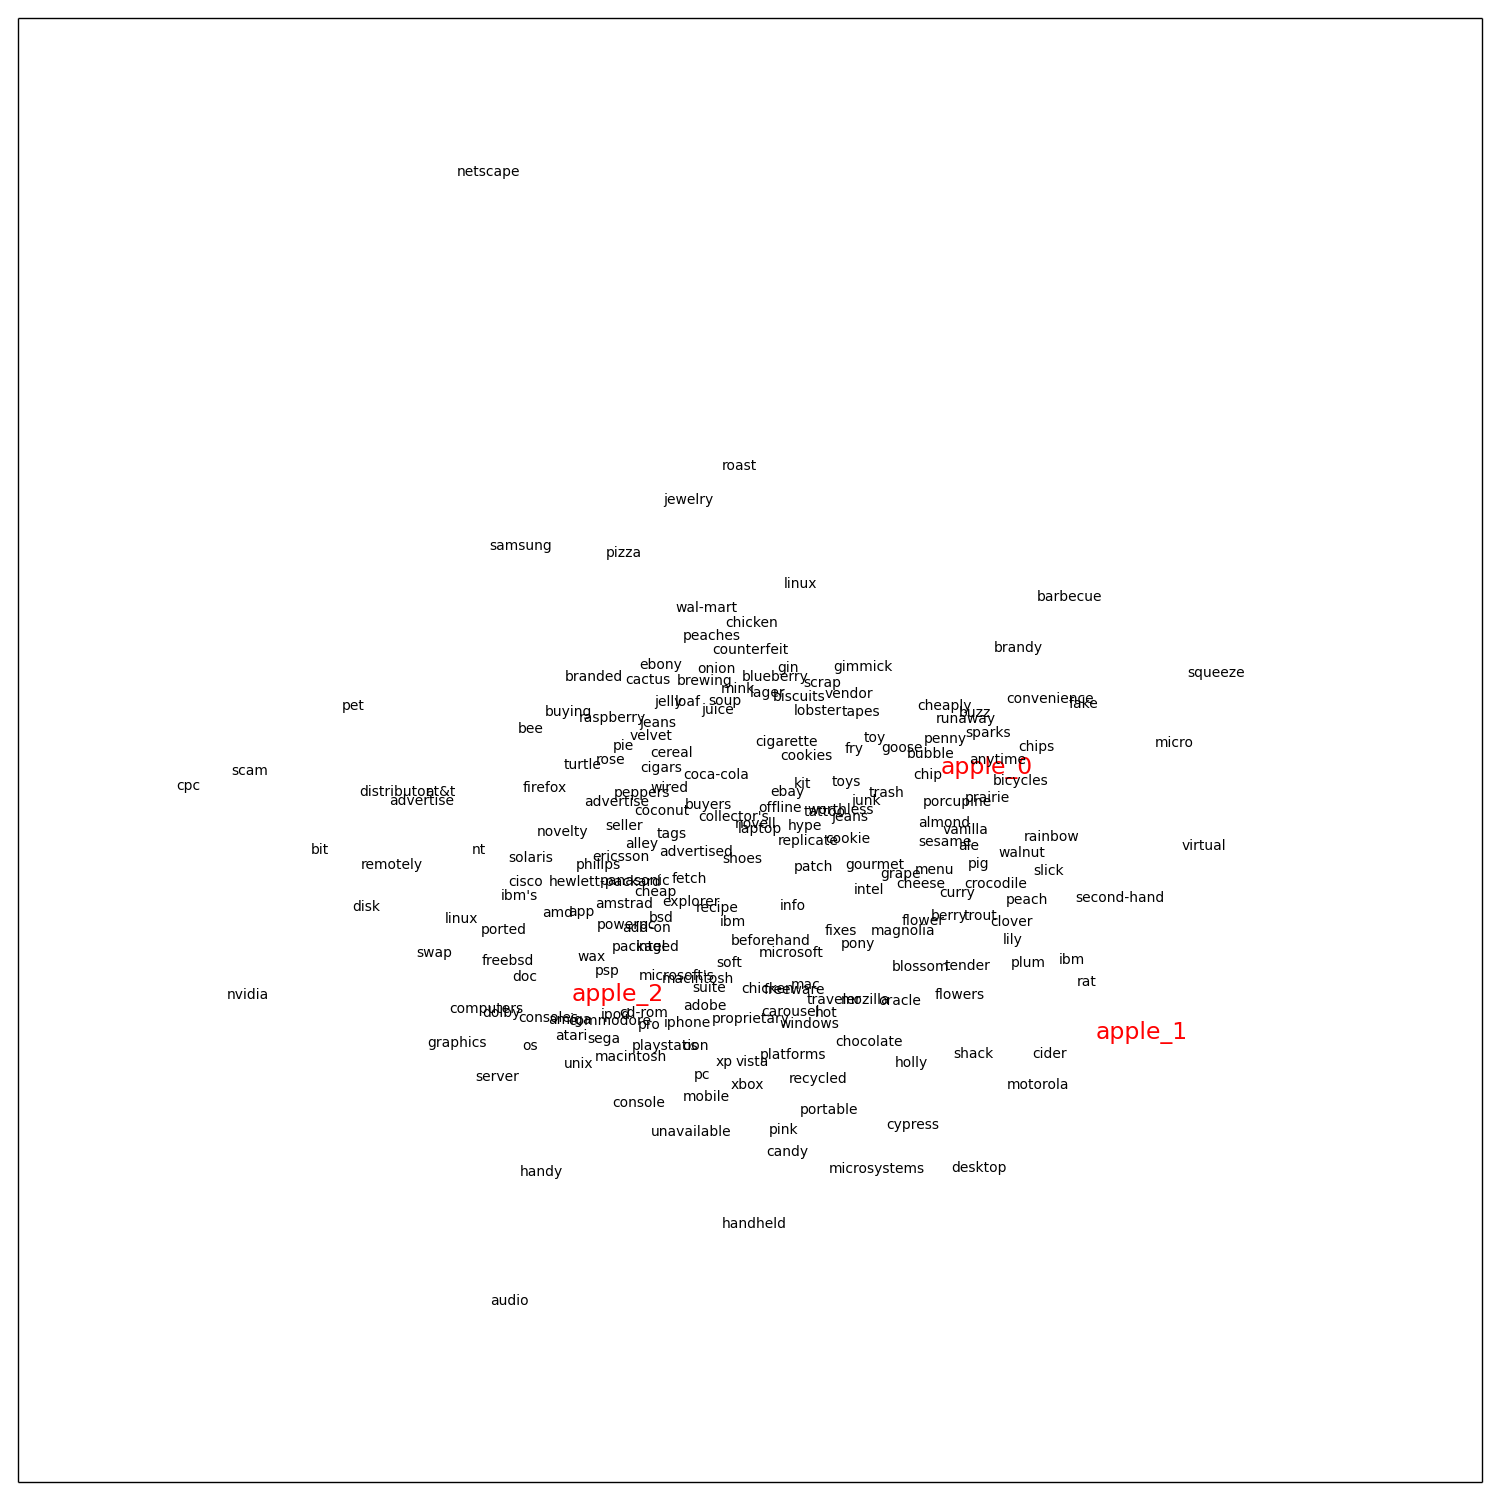
\includegraphics[width=0.8\textwidth]{apple} }
	\caption{Nearest words from $apple$}
	\label{fig:apple}
\end{figure}



\paragraph{} Next, we select other 5 words $fox$ , \ $net$ , \ $rock$ , \ and $plant$, and also list nearest words as Table .. and sentence examples as Table ... in the following. The example sentences are also cut by ourself without affecting the meaning of the sentence. It's not difficult to find that $fox$ has meanings: ; $net$ has meanings: ; $rock$ has meanings: ; $plant$ has meanings: . 


\begin{center} \begin{tabular}{l*{6}{c}r}  $fox_0$ & archie& potter& wolfe& hitchcock& conan& burnett& savage  \\ $fox_1$ & buck& housewives& colbert& eastenders& howard& kane& freeze
 \\ $fox_2$ & abc& sky& syndicated& cw& network's& ctv& pbs \\ \end{tabular} \end{center}

\begin{center} \begin{tabular}{l*{6}{c}r}   $net_0$: & generates& atm& footprint& target& kbit/s& throughput& metering   \\  $net_1$: & trillion& rs& earnings& turnover& gross& euros& profit  
 \\  $net_2$: &jumped& rolled& rebound& ladder& deficit& snapped& whistle   \\  \end{tabular} \end{center}
 
\begin{center} \begin{tabular}{l*{6}{c}r}   $rock_0$: &echo& surf& memphis& strawberry& clearwater& cliff& sunset  \\  $rock_1$: & r$\&$b& hip& roll& indie& ska& indie& hop  
 \\  $rock_2$: &formations& crust& melting& lava& boulders& granite& dust   \\  \end{tabular} \end{center}
 
 \begin{center} \begin{tabular}{l*{6}{c}r}   $run_0$: & blair& taft& fraser& monroe& precinct& mayor's& governor's  \\  $run_1$: & streak& rushing& tying& shutout& inning& wicket& kickoff
 \\  $run_2$: &running& tram& travel& express& trams& inbound& long-distance \\  \end{tabular} \end{center}
 
 \begin{center} \begin{tabular}{l*{6}{c}r}   $plant_0$: &plants& insect& seeds& seed& pollen& aquatic& organic  \\  $plant_1$: &flowering& orchid& genus& bird& species& plants& butterfly
 \\  $plant_2$: &electricity& steel& refinery& refinery& manufacturing& gas& turbine  \\  \end{tabular} \end{center}

\begin{table}
\begin{center} 
\begin{tabular}{|l|l|}
\hline
\multirow{3}{*}{$fox$} 
&run by nathaniel mellors dan \textcolor{red}{$fox_0$} andy cooke and ashley marlowe\\
&he can box like a \textcolor{red}{$fox_1$} he's as dumb as an ox\\
&the grand final was replayed on fox sports australia and the \textcolor{red}{$fox_2$} footy channel\\
\hline
\multirow{3}{*}{$net$} 
&\textcolor{red}{$net_0$} supports several disk image formats partitioning schemes\\
&in mr cook was on the forbes with a \textcolor{red}{$net_1$} worth of billion \\
&nothin but \textcolor{red}{$net_2$} freefall feet into a net below story tower\\
\hline
\multirow{3}{*}{$rock$} 
&zero nine is a finnish hard \textcolor{red}{$rock_0$} band formed in kuusamo in\\
&matt ellis b december is a folk \textcolor{red}{$rock_1$} genre singer-songwriter\\
&cabo de natural park is characterised by volcanic \textcolor{red}{$rock_2$} formations\\
\hline
\multirow{3}{*}{$run$} 
&dean announced that she intends to \textcolor{red}{$run_0$} for mayor again in the november election\\
& we just couldn't \textcolor{red}{$run_1$} the ball coach tyrone willingham said\\
& the terminal is \textcolor{red}{$run_2$} by british rail freight company ews\\
\hline
\multirow{3}{*}{$plant$} 
&these phosphoinositides are also found in \textcolor{red}{$plant_0$} cells with the exception of pip\\
&is a genus of flowering \textcolor{red}{$plant_1$} in the malvaceae sensu lato\\
&was replaced with a new square-foot light fixture \textcolor{red}{$plant_2$} in sparta tn\\
\hline
\end{tabular} 
\caption{Sentence Examples of $apple$} \label{tab:sentenceapple} 
\end{center}
\end{table}


\paragraph{} In the last, for each sense of each word ($apple$, $fox$,$net$,$rock$ and $plant$), we select only 20 nearest words, and combine them together to do another t-SNE embedding, which is also two dimension. The the result is shown in Figure \ref{fig:keywords20}. 

\begin{figure}[!ht]
  \centering
	\fbox{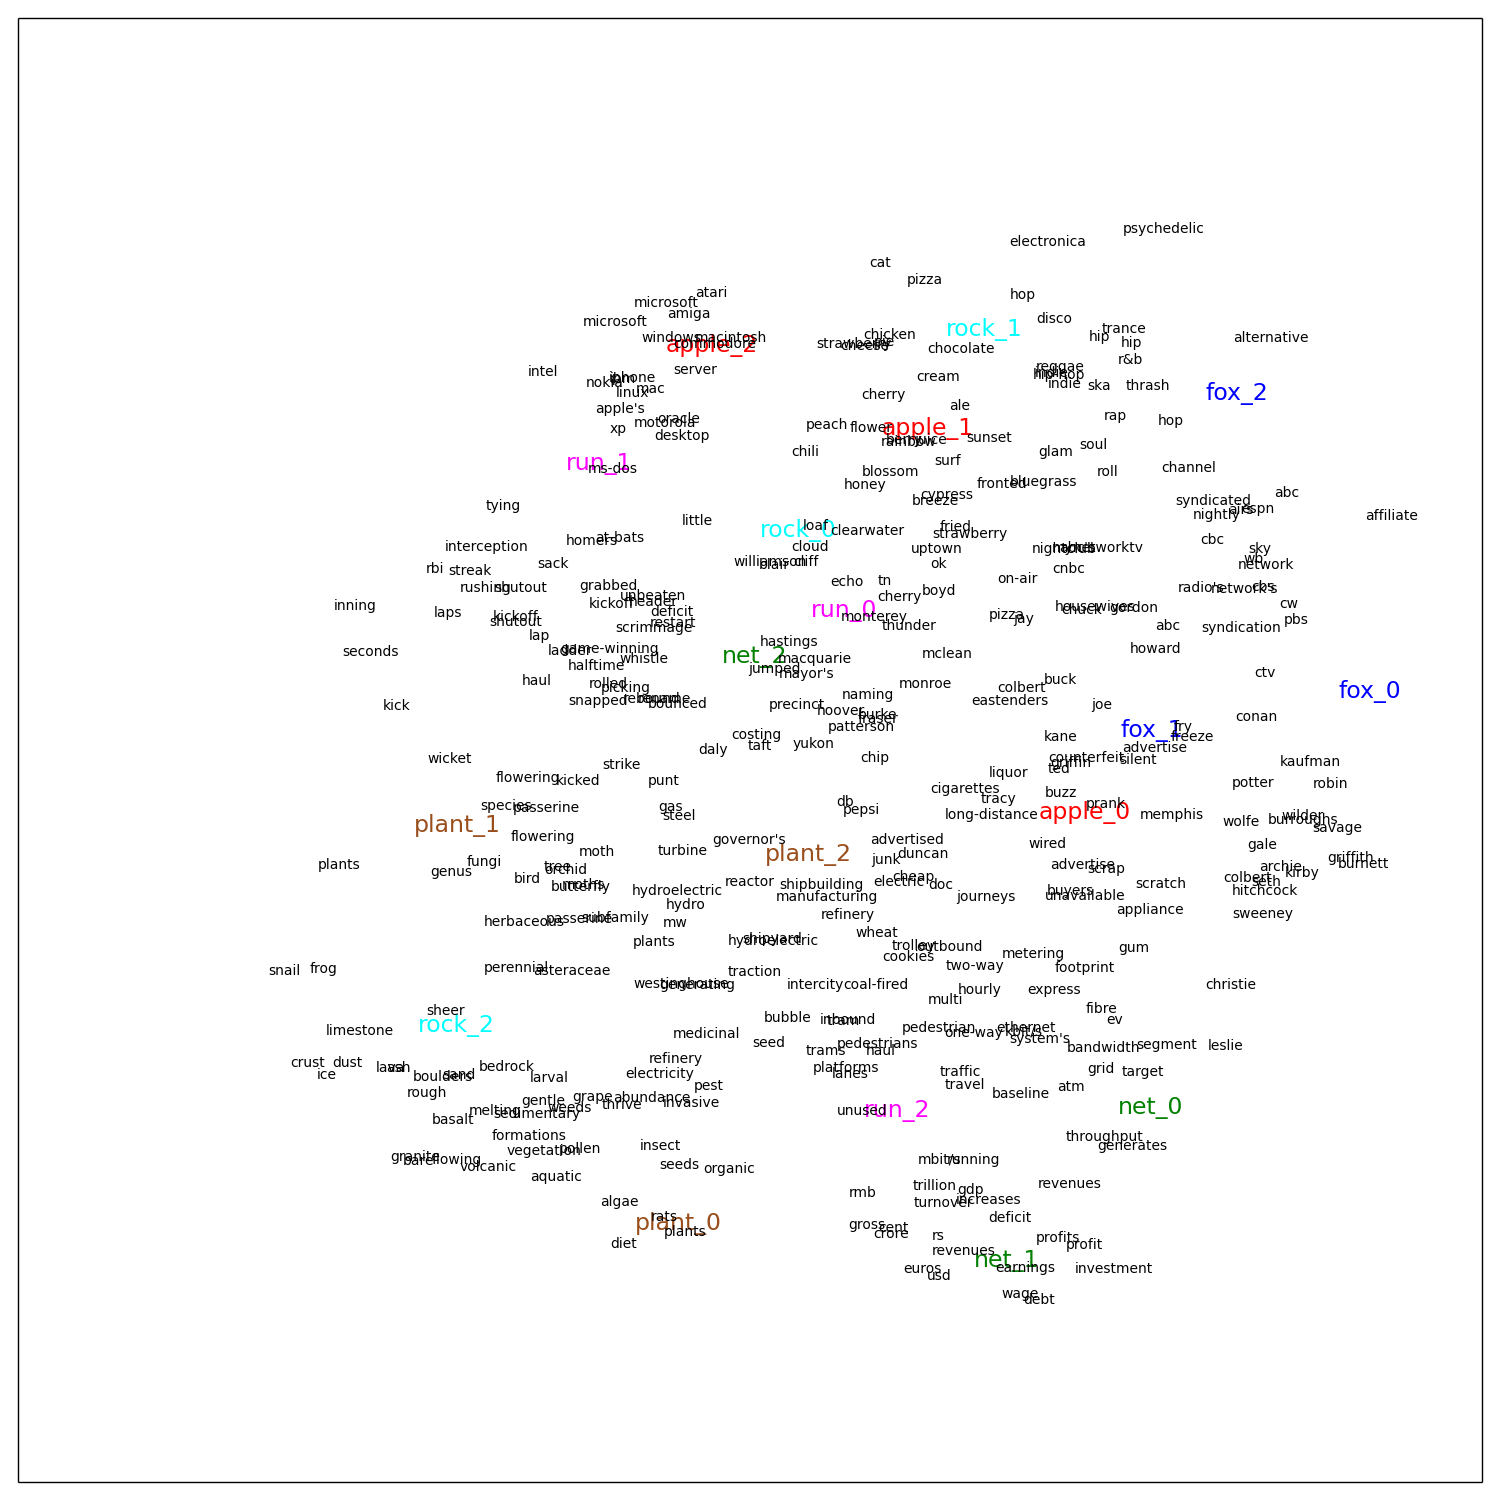
\includegraphics[width=0.9\textwidth]{some20} }
	\caption{Nearest words from 5 key words: $apple$,\ ,$fox$,\ ,$net$,\ ,$rock$,\  , $run$ and $plant$}
	\label{fig:keywords20}
\end{figure}

\paragraph{} From the above results, we can say our model is successful to get multiple senses vectors.
